\subsection{Discussion}  
We make a number of assumptions and choices in our \eda~prescription. 
First, we use the slab model (Eq.~\ref{eq:slab}) to assign $A_V$ as a
function of $\tau_V$ and randomly sampled $i$. 
This choice is motivated by the fact that the slab model reproduces
the correlation between attenuations and inclination found in star-forming
galaxies from observations~\citep{conroy2010b, wild2011, battisti2017,
salim2020} as well as simulations~\citep[\eg][]{chevallard2013,
narayanan2018, trayford2020}.
More importantly, the slab model can reproduce the $A_V$ distribution of
SDSS star-forming galaxies as well as the GSWLC2 sample, which includes
quiescent galaxies (Appendix~\ref{sec:slab}).
We therefore conclude that we can sample $A_V$ in our \eda~with sufficient
flexibility using the slab model. 
%It can also reproduce the SDSS $A_V$ distribution (Figure~\ref{fig:av_dist}). If we replace the slab model with a more flexible model for sampling $A_V$ using truncated normal distributions, we find that our results are not significantly impacted (see Appendix~\ref{sec:slab} for details). Therefore, we conclude that our results do not sigificantly depend on our choice of the slab model. 

In our \eda, we also use a parameterization of $\tau_V$ and $\delta$ that
depend linearly on $\log M_*$ and $\log {\rm SSFR}$. 
While the $M_*$ and $\ssfr$ dependence of $A_V$ is well-motivated and is
found in, for instance, the \cite{salim2018} GSWLC2 catalog (Appendix~\ref{sec:slab}), 
the linear dependence was chosen primarily for its simplicity.
The \eda~framework can be easily extended to more flexible
parameterizations. 
\chedit{
    Though we already find good agreement with SDSS observations, a more
    flexible parameterization would likely produce
    even better agreement with the SDSS color-magnitude relations. 
}
%Our \eda~prescription, for instance, produces slightly broader distributions of optical colors than SDSS. 
The main challenges for a more flexible parameterization would be model
selection and finding a well-motivated parameterization. 

% do we want to mention the FUV and NUV absolute magnitude measurements for
% SDSS? 
\chedit{
    We demonstrate in this work that accounting for dust attenuation is
    essential when comparing simulations to observations. 
    After all, none of the simulations reproduce the UV and optical
    color-magnitude relation without dust (Figure~\ref{fig:obs}). 
}
Furthermore, the fact that we can use the \eda~to reproduce SDSS observations 
for different hydrodynamical simulations highlights how our current lack of 
understanding of dust limits our ability to closely compare galaxy
formation models. 
Our \eda~prescription is built on what we currently know about dust attenuation
in galaxies: \eg~the \citealt{noll2009} parameterization, the UV bump, the slab
model, \emph{etc}.
Yet with the \eda, simulations that predict galaxy populations with
significantly different physical properties (Figure~\ref{fig:smf_msfr}) can
reproduce the same SDSS observations. 
\chedit{
    For instance, SIMBA has significantly fewer massive galaxies above $M_* >
    10^{11}M_\odot$ than TNG or EAGLE (see SMFs in Figure~\ref{fig:smf_msfr}). 
    It also has $M_* < 10^{10}M_\odot$ starburst galaxies with $\ssfr >
    10^{-9.5}yr^{-1}$ (see also \citealt{dave2019} Figures~5 and 6)
    that are not found in TNG or EAGLE (Figure~\ref{fig:avmsfr}). 
    Despite these differences, the forward modeled color-magnitude relations of
    SIMBA is able to comparably reproduce SDSS observations, besides the
    luminous UV red galaxies (Figure~\ref{fig:dem})
}

All this suggests that dust is highly degenerate with the differences between simulations. 
Put another way --- if we were to marginalize over dust in our comparison to
observations, we would not be able to differentiate between the different
galaxy physics prescriptions in the simulations. 
Hence, current limitations in our understanding of dust are a major bottleneck
for investigating galaxy formation using simulations.
In the next paper of the series, Starkenburg et al. (in preparation), we
will examine whether we can compare the prescriptions for star formation
quenching in different galaxy formation models once we include the
\eda~framework.


%\chedit{
%    Figure~\ref{fig:avmsfr} also highlights the selection function imposed by
%    our forward model. 
%    We impose a $M_r < -20$, $M_{FUV} < 13.5$, and $M_{NUV} < -14$
%    absolute magnitude completeness limits of our SDSS sample to the
%    observables of each simulation. 
%    The forward modeled samples expectedly include lower mass star-forming
%    galaxies that are more luminous, while they exclude lower mass quiescent
%    galaxies that are less luminous. 
%    While the forward modeled samples of TNG and EAGLE have comparable $M_*$
%    and $\ssfr$ coverage, we find that SIMBA includes a significant population
%    of lower mass star-forming and quiescent galaxies. 
%    One reason for this is that SIMBA has much fewer massive galaxies above
%    $M_* > 10^{11}M_\odot$ than TNG or EAGLE (see SMFs in
%    Figure~\ref{fig:smf_msfr}). 
%    With fewer massive galaxies, SIMBA requires less attenuation for quiescent
%    galaxies and, thus, its forward model includes lower mass quiescent
%    galaxies.
%    Meanwhile, the $M_* < 10^{10}M_\odot$ lower mass star-forming galaxies included in
%    SIMBA are high $\ssfr > 10^{-9.5}yr^{-1}$ starburst galaxies that lie
%    significantly above the SFS (Figure~\ref{fig:smf_msfr}).
%    This starburst population has also been identified in \cite{dave2019} (see
%    their Figures~5 and 6) and is caused by large gas in low-mass galaxies at $z=0$. 
%} 



\begin{figure}
\begin{center}
    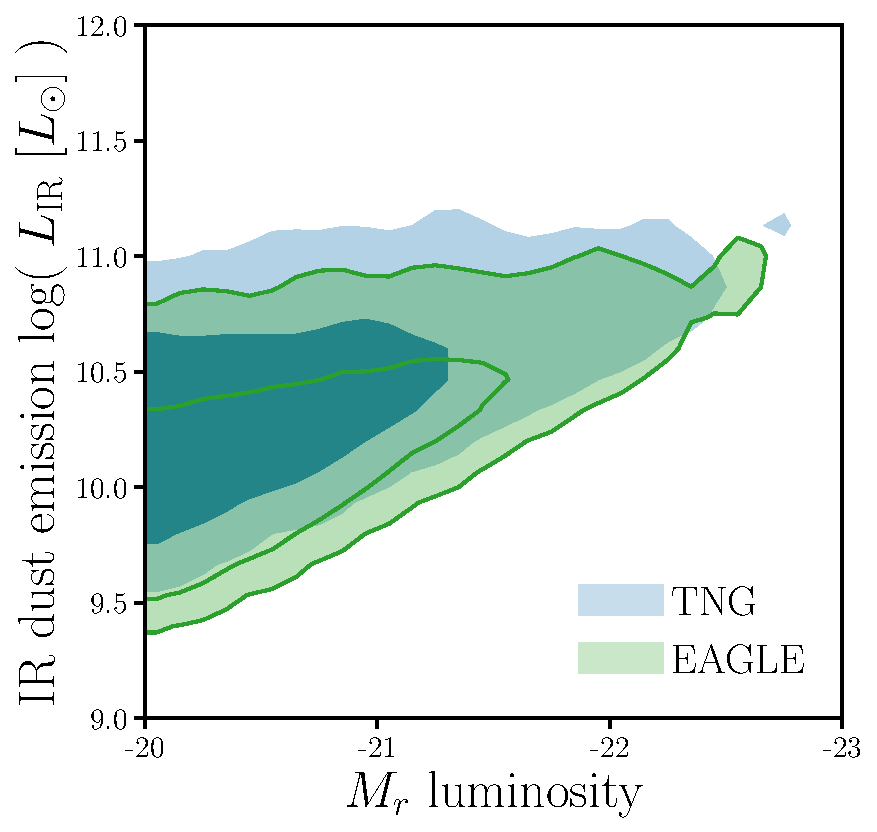
\includegraphics[width=0.45\textwidth]{figs/abc_Lir.pdf}
    \caption{\label{fig:lir}
    IR dust emission luminosity predicted by the \eda~with median parameter
    values of the SIMBA (orange), TNG (blue), and EAGLE (green) posteriors as a
    function of $M_r$. 
    The dust emission is estimated assuming the \cite{dacunha2008} energy balance.
    Despite reproducing the same SDSS UV and optical color-magnitude relations,
    because the simulations require different amounts of dust attenuation to do
    this, \emph{the \eda~predicts significantly different IR dust emissions}.
    Therefore, including IR observations will significantly improve the
    constraints on \eda~parameters and allow us to better differentiate galaxy
    formation models.
    }
\end{center}
\end{figure}

%There's hope! 
Fortunately, there are many avenues for improving our understanding of dust
with a forward modeling approach. 
In this work, we used a restrictive SDSS galaxy sample with a $M_r < -20$,
$M_{FUV} < 13.5$, and $M_{NUV} < -14$ completeness limit. 
\chedit{
    Figure~\ref{fig:avmsfr} illustrates that this selection excludes star-forming
    galaxies below $M_* \lesssim 10^{10}M_\odot$ and quiescent
    galaxies below $M_* \lesssim 10^{10.5}M_\odot$. 
    The $M_*$ limit of the selection is lower for SIMBA due to its lack of massive
    galaxies and low mass starburst galaxies. 
}
Instead of imposing this completeness limit, we can include the actual SDSS
selection function in the forward 
model~\citep[\eg~][]{dickey2020}. 
This would allow us to compare the simulations with \eda~to the entire SDSS
sample, a substantially larger sample with a wider range of galaxies. 
Upcoming surveys, such as the Bright Galaxy Survey (BGS) of the Dark Energy
Spectroscopic Instrument~\citep[DESI;][]{desicollaboration2016, ruiz-macias2020} 
and galaxy evolution survey of the Prime Focus
Spectrograph~\citep[PFS;][]{takada2014,tamura2016}, will vastly expand galaxy
observations. 
BGS, for instance, will measure $10\times$ the number of galaxy spectra as
SDSS out to $z\sim0.4$  and with its $r\sim20$ magnitude limit will probe
a significant number of low redshift dwarf galaxies. 
Such an observational sample will allow us to place tighter constraints on
the \eda~parameters, which may enable comparisons of the underlying galaxy
formation models, and shed light on dust in a broader range of galaxies.
    
In this work, we also only used observables derived from UV and optical
photometry, which means that we have only examined one side of the impact
that dust has on galaxy spectra.
While dust attenuates light in the optical and UV, it emits light in
IR. In fact, even though the simulations reproduce the same SDSS UV and
optical color-magnitude relations with the \eda, they predict significantly 
different dust emission in the IR. 
\chedit{
    In Figure~\ref{fig:lir}, we present IR dust emission luminosity, $L_{\rm
    IR}$, predicted by the \eda~with median parameter values of the SIMBA
    (orange), TNG (blue), and EAGLE (green) posteriors as a function of the
    $r$-band absolute magnitude, $M_r$.
}
The dust emissions are estimated using the standard energy balance assumption
--- \ie~all starlight attenuated by dust is reemitted in the IR~\citep{dacunha2008}. 
\chedit{
    Most noticably, SIMBA and TNG have bimodal distributions of dust emission
    while EAGLE only has luminous IR dust emissions. 
    This is because EAGLE requires significant dust attenuation in all
    galaxies while SIMBA and TNG require quiescent galaxies to have
    substantially lower dust attenuation than star-forming galaxies
    (Figure~\ref{fig:q_raw_atten}). 
    The luminous mode of the $L_{\rm IR}$ distributions, however, are in good
    agreement for all simulations, since they all require comparable dust
    attenuation in star-forming galaxies
    (Figures~\ref{fig:slope} and~\ref{fig:q_raw_atten}). 
    When we compare the IR dust emission of SIMBA+\eda~and TNG+\eda~further, we
    find that TNG+\eda~produces more luminous galaxies with high IR dust
    emission ($M_r < -22$ and $L_{rm IR} > 10^9L_\odot$) since it has more
    intrinsically luminous star-forming galaxies~(Figure~\ref{fig:obs}).
    On the other hand SIMBA+\eda~has more luminous galaxies with fainter IR
    dust emissions, which correspond to the anomolous luminous UV red galaxies
    highlighted in Figure~\ref{fig:uv_sfh}.
}

\chedit{
    While dust attenuation can be adjusted to reproduce UV and optical
    observations, since IR dust emission measures the total attenuation, IR
    observations can place a limit on the total impact of dust and thereby
    break the degeneracies between dust and the galaxy physics in simulations.
}
While some upcoming surveys, such as BGS, will have existing near-IR
photometry from NEOWISE~\citep{meisner2018}, future observations will
dramatically expand the information we have in IR.
\emph{Nancy Grace Roman Space Telescope} and \emph{James Webb Space
Telescope}, for instance, will provide valuable near and
mid-IR observations. 
Meanwhile, IR observations at even longer wavelengths will come from
Atacama Large Millimeter/submillimeter Array or future facilities
such as the Next-Generation Very Large Array and \emph{Origins Space Telescope}.

% Salim(2020): Chevallard et al. (2013), who aggregated and analyzed a diverse series of theoretical attenuation law studies by Pierini et al. (2004), Tuffs et al. (2004), Silva et al. (1998) and Jonsson et al. (2006), and showed that all the stud- ies predict, with some normalization differences, a relationship between the optical depth AV and attenuation law slope.

% Salmon+(2016): There is evidence that galaxy inclination correlates with the strength of Lyα emission, such that we observe less Lyα equivalent width for more edge-on galaxies (Charlot & Fall 1993; Laursen & Sommer-Larsen 2007; Yajima et al. 2012; Verhamme et al. 2012; U et al. 2015)
% Therefore, based on physi- cal models, one expects that galaxies with “greyer” dust laws and larger overall attenuation should have higher inclinations
% Salim+(2018): Chevallard et al. (2013) furthermore show that the depend- ence of the slope on AV is the same irrespective of whether the AV is driven by different levels of intrinsic (face-on) attenuation or is the result of inclined viewing geometry. 


